\clearpage
\mysection{Blague avec le jeu Color Lines}
\label{chap:color_lines}

Ceci est un jeu très répandu dont il existe plusieurs implémentations. Nous utilisons
l'une d'entre elles, appelée BallTriX, de 1997, disponible librement ici \url{https://archive.org/details/BallTriX_1020}
\footnote{Ou ici \url{https://web.archive.org/web/20141110053442/http://www.download-central.ws/Win32/Games/B/BallTriX/} ou \url{http://www.benya.com/balltrix/}.}.
Voici à quoi il ressemble:%

\begin{figure}[H]
\centering
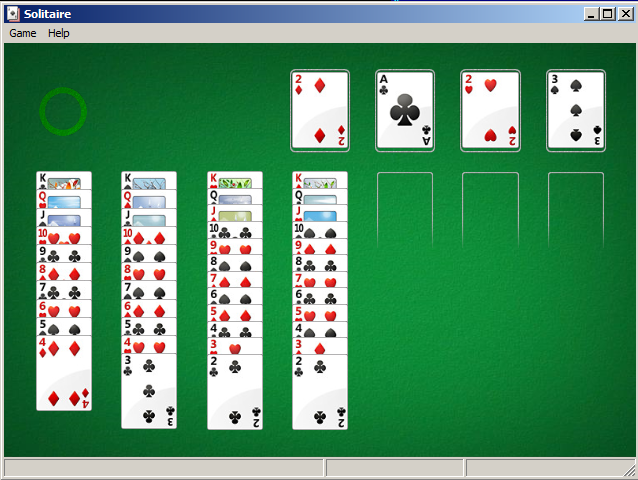
\includegraphics[width=0.6\textwidth]{examples/lines/1.png}
\caption{Ceci est l'allure du jeu en général}
\label{fig:lines_1}
\end{figure}

\clearpage
\myindex{\CStandardLibrary!rand()}

Dons regardons s'il est possible de trouver le générateur d'aléas et de jouer des tours avec.
\IDA reconnaît rapidement la fonction standard \TT{\_rand} dans \TT{balltrix.exe} en \TT{0x00403DA0}.
\IDA montre aussi qu'elle n'est appelée que d'un seul endroit:

\lstinputlisting[style=customasmx86]{examples/lines/random.lst}

Appelons-la \q{random}.
Ne plongeons pas encore dans le code de cette fonction.

Cette fonction est référencée depuis 3 endroits.

Voici les deux premiers:

\lstinputlisting[style=customasmx86]{examples/lines/1.lst}

Voici le troisième:

\lstinputlisting[style=customasmx86]{examples/lines/2.lst}

Donc la fonction n'a qu'un argument.

10 est passé dans les deux premiers cas et 5 dans le troisième.
Nous pouvons aussi remarquer que le plateau a une taille de 10*10, et qu'il y a 5
couleurs possible.
C'est ça!
La fonction standard \TT{rand()} renvoie un nombre dans l'intervalle \TT{0..0x7FFF}
et c'est souvent peu pratique, donc beaucoup de programmeurs implémentent leur propre
fonction qui renvoie un nombre aléatoire dans un intervalle spécifié.
Dans notre cas, l'intervalle est $0..n-1$ et $n$ est passé comme unique argument
à la fonction.
Nous pouvons tester cela rapidement dans le débogueur.

Donc modifions le troisième appel de la fonction, afin qu'il renvoie toujours zéro.
Premièrement, nous allons remplacer trois instructions (\TT{PUSH/CALL/ADD}) par des \ac{NOP}s.
Puis, nous allons ajouter l'instruction \INS{XOR EAX, EAX} pour effacer le registre
\EAX.

\lstinputlisting[style=customasmx86]{examples/lines/fixed.lst}

Nous avons remplacé l'appel à la fonction \TT{random()} par du code qui renvoie toujours
zéro.

\clearpage
Lançons-le maintenant:

\begin{figure}[H]
\centering
\includegraphics[width=0.6\textwidth]{examples/lines/2.png}
\caption{La blague fonctionne}
\end{figure}

Hé oui, ça fonctionne\footnote{J'ai fait une fois cette blague à des collègues dans
l'espoir qu'ils arrêtent de jouer. Mais ça n'a pas fonctionné.}.

Mais pourquoi est-ce que les arguments de la fonction \TT{random()} sont des variables
globales?
C'est seulement parce qu'il est possible de changer la taille du plateau dans les
préférences du jeu, donc ces valeurs ne sont pas codées en dur.
Le valeurs 10 et 5 sont celles par défaut.
